\documentclass[10pt]{article}

\usepackage[utf8x]{inputenc}
\usepackage[T1]{fontenc}
\usepackage{amsfonts,amsmath,amssymb,amsthm,booktabs,color,graphicx}
\usepackage[ruled,vlined,linesnumbered]{algorithm2e}
\usepackage{enumitem}

\newtheorem{lemma}{Lemma}

\title{String Processing Algorithms 2015 - Week 2 Exercises}
\author{Rodion Efremov}
\date{\today}

\begin{document}
\maketitle

\section*{Exercise 1}
\color{blue} Outline algorithms that find the most frequent symbol in a give string.
\begin{enumerate}[label=(\alph*)]
\item for ordered alphabet, and
\item for integer alphabet.
\end{enumerate}
The algorithms should be as fast as possible. What are their (worst case) time complexities?  Consider also the case where $\sigma \gg n$. \color{black}

\subsection*{Solution}
\begin{algorithm}
\SetKw{KwLet}{let}
\SetKw{KwEmptyMap}{be an empty map}
\SetKw{KwNil}{nil}
\SetKw{KwNotMapped}{is not mapped in}
\KwLet $f$ \KwEmptyMap $f \colon \Sigma \to \mathbb{N}$ \\
$\mu = $ \KwNil \\
$L_{\mu} = 0$ \\
\For{$i = 1$ \KwTo $|S|$}{
	\If{$S[i]$ \KwNotMapped $f$}{
	    $f(S[i]) = 1$ \\
	    
	    \If{$L_{\mu} = 0$}{
	      $L_{\mu} = 1$ \\
	      $\mu = S[i]$ \\
	    }
	} \Else{
      $f(S[i]) = f(S[i]) + 1$ \\
      
      \If{$L_{\mu} < f(S[i])$}{
        $L_{\mu} = f(S[i])$ \\
        $\mu = S[i]$ \\
      }	
	}
}
\KwRet $\mu$ \\ 
\caption{\textsc{MostFrequentSymbol}$(S)$}
\end{algorithm}

\section*{Exercise 2}
\color{blue} Let $\mathcal{R} = \{ \texttt{manne}, \texttt{manu}, \texttt{minna}, \texttt{salla},\texttt{saul}, \texttt{sauli}, \texttt{vihtori} \}$.
\begin{enumerate}[label=(\alph*)]
\item Give the compact trie of $\mathcal{R}$.
\item Give the balanced compact ternary trie of $\mathcal{R}$.
\end{enumerate}
\color{black}

\subsection*{Solution}
\subsubsection*{(a)}
\begin{center}
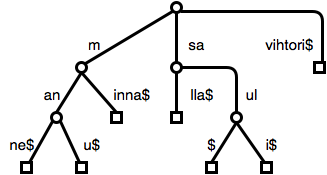
\includegraphics[scale=0.65]{CompactTrie}
\end{center}

\subsubsection*{(b)}
\begin{center}
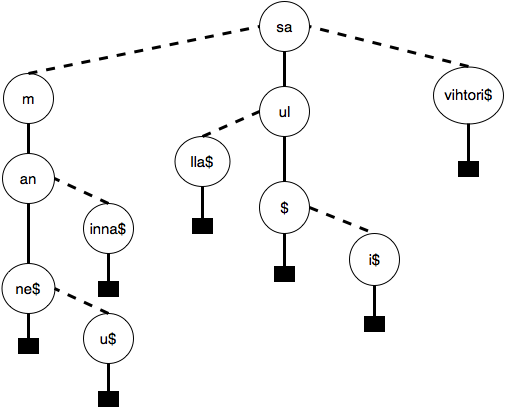
\includegraphics[scale=0.65]{TernaryTrie}
\end{center}

\section*{Exercise 3}

\section*{Exercise 4}
\color{blue}
Prove
\begin{enumerate}[label=(\alph*)]
\item Lemma 1.14: For $i \in [2..n]$, $LCP_{\mathcal{R}}[i] = lcp(S_i, \{ S_1, \dots, S_{i - 1} \})$.
\item Lemma 1.15: $\Sigma LCP(\mathcal{R}) \leq \Sigma lcp(\mathcal{R}) \leq 2 \cdot \Sigma LCP(\mathcal{R})$.
\end{enumerate}
\color{black}
\subsection*{Solution}

\subsubsection*{(a)}
We need an auxiliary lemma first: 
\begin{lemma}[Distance lemma]
If $S_1 < S_2 < S_3$, $lcp(S_1, S_3) \leq lcp(S_2, S_3)$.
\end{lemma}
\begin{proof}
The proof is by contradiction: Let $l_{13} = lcp(S_1, S_3)$ and $l_{23} = lcp(S_2, S_3)$. Assume the opposite that $l_{13} > l_{23}$. 
Now 
\begin{align*}
S_1 &= a_1 a_2 \dots a_{l_{23}} \dots a_{l_{13}} b_1 b_2 \dots, \\
S_2 &= a_1 a_2 \dots a_{l_{23}} c_1 c_2 \dots, \\
S_3 &= a_1 a_2 \dots a_{l_{23}} \dots a_{l_{13}} d_1 d_2 \dots.
\end{align*}
Since $c_1 > a_{l_{23} + 1}$, we must have also $S_2 > S_3$, which is a contradiction.
\end{proof}
\subsubsection*{Example:}
\begin{align*}
S_1: & aaaab \\
S_2: & aaaba \\
S_3: & aaabc
\end{align*}
Now assume that $i \in [2...n]$. We have that
\begin{align*}
lcp(S_i, \{ S_1, \dots, S_{i - 1} \}) &= \max \{ lcp(S_i, S_{i - 1}), lcp(S_i, \{ S_1, \dots, S_{i - 2} \}) \}.
\end{align*}
Because by distance lemma for any $j = 1, 2, \dots, i - 2$, $lcp(S_j, S_i)$ cannot exceed $lcp(S_i, S_{i - 1})$, we must have that 
\[
lcp(S_i, \{ S_1, \dots, S_{i - 1} \}) = lcp(S_i, S_{i - 1}) = LCP_{\mathcal{R}}[i],
\] 
as expected.

\subsubsection*{(b)}
\begin{align*}
\Sigma lcp(\mathcal{R}) &= \sum_{S \in \mathcal{R}} lcp(S, \mathcal{R} \setminus \{ S \}) \\
									  &\leq \sum_{i \in [1 .. n - 1]} lcp(S_i, S_{i + 1}) + \sum_{i \in [2 .. n]} lcp(S_{i - 1}, S_i) &\text{\quad (by distance lemma)} \\
									  &= \sum_{i \in [2 .. n]} lcp(S_{i - 1}, S_i) + \sum_{i \in [2 .. n]} lcp(S_{i - 1}, S_i) \\
									  &= 2 \sum_{i \in [2 .. n]} lcp(S_{i - 1}, S_i) \\
									  &= 2 \sum_{i \in [2 .. n]} LCP_{\mathcal{R}}[i] \\
									  &= 2 \sum_{i \in [1 .. n]} LCP_{\mathcal{R}}[i] & \text{\quad (since } LCP_{\mathcal{R}}[1] = 0) \\
									  &= 2 \cdot \Sigma LCP(\mathcal{R}).
\end{align*}
What comes to the lower bound of $\Sigma lcp(\mathcal{R})$, we have
\begin{align*}
\Sigma lcp(\mathcal{R}) &= lcp(S_1, S_2) + lcp(S_{n - 1}, S_n) \\
 									  &+ \sum_{i \in [2 .. n - 1]} \max \{ lcp(S_i, S_{i - 1}), lcp(S_i, S_{i + 1}) \} &\text{\quad (by distance lemma)} \\
    								  &\geq \sum_{i \in [2 .. n]} lcp(S_{i - 1}, S_i) \\
    								  &= \sum_{i \in [2 .. n]} LCP_{\mathcal{R}}[i] \\
    								  &= \sum_{i \in [1 .. n]} LCP_{\mathcal{R}}[i] & \text{\quad (since } LCP_{\mathcal{R}}[1] = 0) \\
    								  &= \Sigma LCP(\mathcal{R}),
\end{align*}
which concludes the proof.

\subsubsection*{Example:}
\begin{tabular}{|c|c|c|}
\hline
$\mathcal{R}$ & $LCP_{\mathcal{R}}$ & $lcp(S, \mathcal{R})$ \\
\hline
aaaa & 0 & 3 \\
aaab & 3 & 3 \\
abba & 1 & 1 \\
baab & 0 & 0 \\
\hline
$\sum$ & 4 & 7 \\
\hline
\end{tabular}
\end{document}